%%%%%%%%%%%%%%%%%%%%%%%%%%%%%%%%%%%%%%%%%%%%%%%%%%%%%%%%%%%%%%%%
%                                                              %
% This is a LaTeX file.  It is a text file that is compiled    %
% by a program called LaTeX into a pretty PDF file.            %
% If you're viewing this file on Overleaf,                     %
% you'll see that PDF in the window to the right.              %
%                                                              %
% The LaTeX macro language is complicated, so we have inserted %
% lots of documenting comments into the file.  Comments start  %
% with `%' and continue to the end of the line.                %
%                                                              %
% Comments are provided to let you, the student, understand    %
% what that part of the code is doing or to provide you with   %
% instructions.                                                % 
%                                                              %
% Skip anything else you don't understand, or ask me.          %
%                                                              %
%%%%%%%%%%%%%%%%%%%%%%%%%%%%%%%%%%%%%%%%%%%%%%%%%%%%%%%%%%%%%%%%
%
\documentclass{article}
\usepackage[left=1in,right=1in,top=1in,bottom=1in]{geometry}
% 
%%%%%%%%%%%%%%%%%%%%%%%%%%%%%%%%%%%%%%%%%%%%%%%%%%%%%%%%%%%%%%%%
%                                                              %
% This is the preamble of the document. This is where we       %
% declare the packages we need for the pdf file to compile     %
% correctly. Packages contain the different commands we        %
% need to use that allow us to format the document nicely.     %
%                                                              %
% You shouldn't need to edit any of these packages.            %
%                                                              %
%%%%%%%%%%%%%%%%%%%%%%%%%%%%%%%%%%%%%%%%%%%%%%%%%%%%%%%%%%%%%%%%
% 
\usepackage{amsmath, amsthm, amsfonts} % These packages contain most of the commands needed to format the maths symbols.
\usepackage{enumerate} % Package that contains options for the \begin{enumerate} environment.
\usepackage{hyperref} % Package that allows hyperlinks.
\usepackage{tikz} % Package that lets us draw diagrams
\newtheorem*{theorem}{Theorem} % Defines an environment with the heading "Theorem". The * supresses the numbering.
\newtheorem*{claim}{Claim} % Defines an environment with the heading "Claim". The * supresses the numbering.
\theoremstyle{definition}
\newtheorem*{definition}{Definition} % Defines an environment with the heading "Definition". The * supresses the numbering.
\newtheorem*{proposition}{Proposition} % Defines an environment with the heading "Proposition". The * supresses the numbering.
\newenvironment{solution}{\bigskip\hrule{\hfill}}{\bigskip\hrule{\hfill}} % Defines an environment that draws lines to make clear where your solution starts and ends.
% 
%%%%%%%%%%%%%%%%%%%%%%%%%%%%%%%%%%%%%%%%%%%%%%%%%%%%%%%%%%%%%%%%
%                                                              %
% In the author command below, type in your name. The article  %
% class will produce a title page using the command \maketitle %
% containing the title of the document, the author name and    %
% the date.                                                    %
%                                                              %
%%%%%%%%%%%%%%%%%%%%%%%%%%%%%%%%%%%%%%%%%%%%%%%%%%%%%%%%%%%%%%%%
%
\title{\textbf{MATH-UA 120 Discrete Mathematics: \\ Problem Set 3}}
\author{%
    Wendy Darling % Change to your name!
}
\date{Due Monday, October 7th, 2024} % The due date of the assignment. All assignemets are dues at 11:59pm on the date listed
%
%%%%%%%%%%%%%%%%%%%%%%%%%%%%%%%%%%%%%%%%%%%%%%%%%%%%%%%%%%%%%%%%
%                                                              %
% The body of the document is typed in between the lines       %
% \begin{document} and \end{document}.                         %
%                                                              %
%%%%%%%%%%%%%%%%%%%%%%%%%%%%%%%%%%%%%%%%%%%%%%%%%%%%%%%%%%%%%%%%
%
\begin{document}
\maketitle % This command generate the title page information that was filled in in the preamble

\vfill

% The following are the asignment instructions. You should leave these alone and, after reading them, proceed to the problems.
\section*{Assignment Instructions}

\begin{itemize}
    \item These are to be written up in \LaTeX{} and turned in on Gradescope.
    \item \href{https://bit.ly/3Tb7ZMc}{\textbf{Click here to duplicate this \texttt{.tex} file in Overleaf}}.
    \item Write your solutions inside the \texttt{solution} environment.
    \item You are always encouraged to talk problems through with your peers and your instructor, but your write up should be done independently.
    \item Problems are graded on correctness and fluency.
    \item Unless stated otherwise, all calculations require justification.
    \item Some tutorials on how to use \LaTeX{} can be found \href{https://www.overleaf.com/learn/latex/Tutorials}{\underline{here}}. If you have any questions about \LaTeX{} commands you can always ask your instructor for advice.
\end{itemize}

\vfill

\section*{Statement on generative AI}

In this and other mathematics courses, you are expected to construct clear and concise mathematical arguments based on statements proven in our text and class notes. Large language models such as ChatGPT are unable to produce this kind of solution. They also frequently generate circular logic and outright false results.
 
You may use AI to summarise content, generate study plans, create problems, or do other study-related activities. You may not ask a chatbot to solve your quiz or homework problems, or do any assessment-related activities.
 
You may use AI tools to edit your grammar and punctuation, but remember that mathematical English is not the same as academic English in other disciplines. 

\vfill

\newpage

%%%%%%%%%%%%%%%%%%%%%%%%%%%%%%%%%%%%%%%%%%%%%%%%%%%%%%%%%%%%%%%%
%%%%%                       Problem 1                      %%%%%
%%%%%%%%%%%%%%%%%%%%%%%%%%%%%%%%%%%%%%%%%%%%%%%%%%%%%%%%%%%%%%%%

\section*{Problem 1}
\begin{enumerate}[a)] % The enumerate environment produces a numbered list of items. The [a)] ensures that the items are labelled with letters instead.
    \item Consider the following subsets of $\mathbb{N}$.
    \begin{align*}
        A & = \text{The set of all even numbers.} \\
        B & = \text{The set of all prime numbers.} \\
        C & = \text{The set of all perfect squares.} \\
        D & = \text{The set of all multiples of }10.
    \end{align*}
    Using only the symbols $$3,A,B,C,D,\mathbb{N},\in,\subseteq,=,\neq,\cap,\cup,\times,-,\emptyset,(,)$$ rewrite the following statements in set notation.
    \begin{enumerate}[i.] % The enumerate environment produces a numbered list of items. The [a)] ensures that the items are labelled with Roman numerals instead.
        \item None of the perfect squares are prime numbers.
        \item The number $3$ is a prime number that is not even.
        \item If you take all of the prime numbers, all of the even numbers, all of the perfect squares and all of the multiples of $10$, you still won't have all of the natural numbers.
    \end{enumerate}
    \item Consider the following subsets of the set of all students at a university.
    \begin{align*}
        F & = \text{The set of all freshmen}. \\
        S & = \text{The set of all seniors}. \\
        M & = \text{The set of all maths majors}. \\
        C & = \text{The set of all CS majors}. 
    \end{align*}
    \begin{enumerate}[i.] % The enumerate environment produces a numbered list of items. The [a)] ensures that the items are labelled with Roman numerals instead.
        \item Using only the symbols $$F,S,M,C,\left|~\right|,\cap,\cup,-,>$$ translate the following statement written in English into a statement written in the language of set theory: ``There are more freshmen that aren't maths majors that there are senior CS majors.''
        \item Translate the following statement written in the language of set theory into a statement in English: $\left(F\cap M\right)\subseteq C$.
    \end{enumerate}
\end{enumerate}
\begin{solution}

% Type your solution to Problem 1 here.

\end{solution}

%%%%%%%%%%%%%%%%%%%%%%%%%%%%%%%%%%%%%%%%%%%%%%%%%%%%%%%%%%%%%%%%

\newpage

%%%%%%%%%%%%%%%%%%%%%%%%%%%%%%%%%%%%%%%%%%%%%%%%%%%%%%%%%%%%%%%%
%%%%%                       Problem 2                      %%%%%
%%%%%%%%%%%%%%%%%%%%%%%%%%%%%%%%%%%%%%%%%%%%%%%%%%%%%%%%%%%%%%%%

\section*{Problem 2}
Describe explicitly in English the following sets, then find their cardinality.
\begin{enumerate}[a)] % The enumerate environment produces a numbered list of items. The [a)] ensures that the items are labelled with letters instead.
    \item $\left\{x\in 2^{\mathbb{Z}}\mid 5\in x\right\}$
    \item $\left\{x\in 2^{\mathbb{Z}}\mid x\subseteq\{1,2,3\}\right\}$
    \item $\left\{x\in 2^{\mathbb{Z}}\mid x\subset\{1,2,\{3,4\}\}\right\}$
    \item $\left\{x\in 2^{\mathbb{Z}}\mid x\in\{1,2,\{3,4\}\}\right\}$
    \item $\left\{x\in 2^{\mathbb{Z}}\mid y\in x\Longrightarrow y=0\right\}$
\end{enumerate}
\begin{solution}

% Type your solution to Problem 2 here.

\end{solution}

%%%%%%%%%%%%%%%%%%%%%%%%%%%%%%%%%%%%%%%%%%%%%%%%%%%%%%%%%%%%%%%%

\newpage

%%%%%%%%%%%%%%%%%%%%%%%%%%%%%%%%%%%%%%%%%%%%%%%%%%%%%%%%%%%%%%%%
%%%%%                       Problem 3                      %%%%%
%%%%%%%%%%%%%%%%%%%%%%%%%%%%%%%%%%%%%%%%%%%%%%%%%%%%%%%%%%%%%%%%

\section*{Problem 3}
For each of the following statements, describe it in English and say if is true or false (without proof). Then write its negation using quantifiers and describe this negation in English. \medskip

\noindent For example: The statement $\forall x\in\mathbb{Z},x<0$ means every integer is negative, and it is false. Its negation is $\exists x\in\mathbb{Z},x\geq 0$, which means that there exists a nonnegative integer.

\begin{enumerate}[a)] % The enumerate environment produces a numbered list of items. The [a)] ensures that the items are labelled with Roman numerals instead.
    \item $\forall x\in\mathbb{Z},~\exists y\in\mathbb{Z},~x^2+y=4$
    \item $\exists y\in\mathbb{Z},~\forall x\in\mathbb{Z},~x^2+y=4$
    \item $\forall n\in\mathbb{Z},~\exists k\in\mathbb{Z},~\exists d\in\mathbb{Z},~k+n=2d$
    \item $\exists n\in\mathbb{Z},~\forall k\in\mathbb{Z},~\exists d\in\mathbb{Z},~k+n=2d$
\end{enumerate}
\begin{solution}

% Type your solution to Problem 3 here.

\end{solution}

%%%%%%%%%%%%%%%%%%%%%%%%%%%%%%%%%%%%%%%%%%%%%%%%%%%%%%%%%%%%%%%%

\newpage

%%%%%%%%%%%%%%%%%%%%%%%%%%%%%%%%%%%%%%%%%%%%%%%%%%%%%%%%%%%%%%%%
%%%%%                       Problem 4                      %%%%%
%%%%%%%%%%%%%%%%%%%%%%%%%%%%%%%%%%%%%%%%%%%%%%%%%%%%%%%%%%%%%%%%

\section*{Problem 4}
Proposition 12.4 of the textbook says that for any finite sets $X$ and $Y$, we have $$\left|X\right|+\left|Y\right|=\left|X\cup Y\right|+\left|X\cap Y\right|.$$ Use this proposition to show that for any three finite sets $A$, $B$ and $C$ that $$\left|A\cup B\cup C\right|=\left|A\right|+\left|B\right|+\left|C\right|-\left|A\cap B\right|+\left|A\cap C\right|-\left|B\cap C\right|+\left|A\cap B\cap C\right|.$$
\begin{solution}

% Type your solution to Problem 4 here.

\end{solution}

%%%%%%%%%%%%%%%%%%%%%%%%%%%%%%%%%%%%%%%%%%%%%%%%%%%%%%%%%%%%%%%%

\newpage

%%%%%%%%%%%%%%%%%%%%%%%%%%%%%%%%%%%%%%%%%%%%%%%%%%%%%%%%%%%%%%%%
%%%%%                       Problem 5                      %%%%%
%%%%%%%%%%%%%%%%%%%%%%%%%%%%%%%%%%%%%%%%%%%%%%%%%%%%%%%%%%%%%%%%

\section*{Problem 5}
In a survey of soda preference between three brands $A$, $B$ and $C$, it found that $60$ people like $A$, $55$ people like $B$, $40$ people like $C$, $20$ people like both $A$ and $B$, $35$ people like both $B$ and $C$, $15$ people like both $A$ and $C$, and $10$ people like all three sodas. Assuming that everyone likes at least one of the three soda brands, find the following:
\begin{enumerate}[a)] % The enumerate environment produces a numbered list of items. The [a)] ensures that the items are labelled with letters instead.
    \item The number of people who participated in the survey.
    \item The number of people who like soda $B$ only.
    \item The number of people who like sodas $A$ and $C$, but not soda $B$.
    \item The number of people who do not like soda $B$.
\end{enumerate}
\begin{solution}

% Type your solution to Problem 5 here.

\end{solution}

%%%%%%%%%%%%%%%%%%%%%%%%%%%%%%%%%%%%%%%%%%%%%%%%%%%%%%%%%%%%%%%%

\newpage

%%%%%%%%%%%%%%%%%%%%%%%%%%%%%%%%%%%%%%%%%%%%%%%%%%%%%%%%%%%%%%%%
%%%%%                       Problem 6                      %%%%%
%%%%%%%%%%%%%%%%%%%%%%%%%%%%%%%%%%%%%%%%%%%%%%%%%%%%%%%%%%%%%%%%

\section*{Problem 6}
Let $A=\left\{x\in\mathbb{Z}\mid 100\leq x\leq 999\right\}$ and $A_i=\left\{x\in A\mid i^{\text{th}}\text{ digit of }x\text{ is }i\right\}$. Find $\left|A_1\cup A_2\cup A_3\right|$.
\begin{solution}

% Type your solution to Problem 6 here.

\end{solution}

%%%%%%%%%%%%%%%%%%%%%%%%%%%%%%%%%%%%%%%%%%%%%%%%%%%%%%%%%%%%%%%%

\newpage

%%%%%%%%%%%%%%%%%%%%%%%%%%%%%%%%%%%%%%%%%%%%%%%%%%%%%%%%%%%%%%%%
%%%%%                       Problem 7                      %%%%%
%%%%%%%%%%%%%%%%%%%%%%%%%%%%%%%%%%%%%%%%%%%%%%%%%%%%%%%%%%%%%%%%

\section*{Problem 7}
Let $n$ be a positive integer. Give a combinatorial proof of the identity $$3^n-1=1\cdot3^0+2\cdot3^1+2\cdot3^2+\cdots+2\cdot3^{n-1}.$$ You may not manipulate the question algebraically. Only a combinatorial proof will be accepted.
\begin{solution}

% Type your solution to Problem 7 here.

\end{solution}

%%%%%%%%%%%%%%%%%%%%%%%%%%%%%%%%%%%%%%%%%%%%%%%%%%%%%%%%%%%%%%%%

\newpage

%%%%%%%%%%%%%%%%%%%%%%%%%%%%%%%%%%%%%%%%%%%%%%%%%%%%%%%%%%%%%%%%
%%%%%                       Problem 8                      %%%%%
%%%%%%%%%%%%%%%%%%%%%%%%%%%%%%%%%%%%%%%%%%%%%%%%%%%%%%%%%%%%%%%%

\section*{Problem 8}
The \emph{Fibonacci numbers} are a sequence of integers $\left(f_n\right)_{n\in\mathbb{N}}$ defined recursively by $$f_0=1,\quad f_1=1, \quad f_n=f_{n-1}+f_{n-2}\text{ for }n\geq2.$$ The sequence begins $1,1,2,3,5,8,13,\dots$. \bigskip

\noindent Consider the following question: How many different ways are there to tile a $1\times n$ board using only square ($1\times 1$) and domino ($1\times 2$) tiles?
\begin{center}
    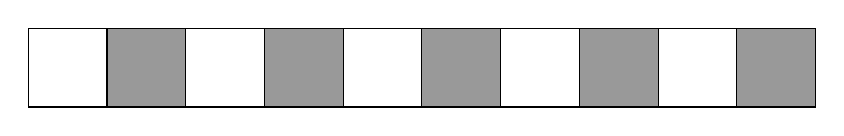
\begin{tikzpicture}
        \def\n{4}
        \draw (0,0) -- (0,1);
        \foreach\x in {0,...,\n}{
            \filldraw[fill=black!40!white] ({2*\x+1},0) -- ({2*\x+2},0) -- ({2*\x+2},1) -- ({2*\x+1},1);
            \draw ({2*\x},0) -- ({2*\x+1},0) -- ({2*\x+1},1) -- ({2*\x},1);
        }
    \end{tikzpicture}
\end{center}

\noindent For example, $1\times1$, $1\times 2$ and $1\times 3$ boards can be tiled in the following ways
\begin{center}
    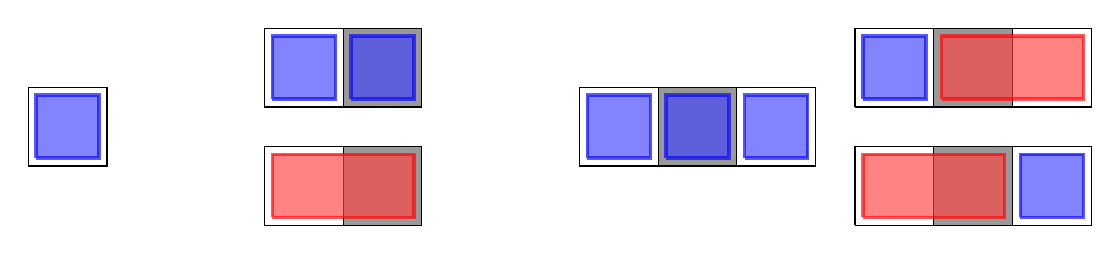
\begin{tikzpicture}
        \def\t{0.1}
        \draw (0,0) -- (0,1) -- (1,1) -- (1,0) -- (0,0);
        \filldraw[very thick,blue,fill=blue!75!white,opacity=0.65] ({0+\t},{0+\t}) -- ({0+\t},{1-\t}) -- ({1-\t},{1-\t}) -- ({1-\t},{0+\t}) -- ({0+\t},{0+\t});
        \def\n{0}\def\X{3}
        \draw ({\X},-0.75) -- ({\X},0.25); \draw ({\X},0.75) -- ({\X},1.75);
        \foreach\y in {-0.75,0.75}{\foreach\x in {0,...,\n}{
            \filldraw[fill=black!40!white] ({\X+\x+1},{\y}) -- ({\X+\x+2},{\y}) -- ({\X+\x+2},{\y+1}) -- ({\X+\x+1},{\y+1});
            \draw ({\X+\x},{\y}) -- ({\X+\x+1},{\y}) -- ({\X+\x+1},{\y+1}) -- ({\X+\x},{{\y+1}});
        }}
        \foreach\x in {0,1}{
            \filldraw[very thick,blue,fill=blue!75!white,opacity=0.65] ({\X+\x+\t},{0.75+\t}) -- ({\X+\x+\t},{1.75-\t}) -- ({\X+\x+1-\t},{1.75-\t}) -- ({\X+\x+1-\t},{0.75+\t}) -- ({\X+\x+\t},{0.75+\t});
        }
        \filldraw[very thick,red,fill=red!75!white,opacity=0.65] ({\X+\t},{-0.75+\t}) -- ({\X+\t},{0.25-\t}) -- ({\X+2-\t},{0.25-\t}) -- ({\X+2-\t},{-0.75+\t}) -- ({\X+\t},{-0.75+\t});
        \def\X{7}
        \draw ({\X},0) -- ({\X},1);
        \foreach\x in {0,...,\n}{
            \filldraw[fill=black!40!white] ({\X+\x+1},{0}) -- ({\X+\x+2},{0}) -- ({\X+\x+2},{1}) -- ({\X+\x+1},{1});
            \draw ({\X+\x},{0}) -- ({\X+\x+1},{0}) -- ({\X+\x+1},{1}) -- ({\X+\x},{{1}});
        }
        \draw ({\X+\n+2},{0}) -- ({\X+\n+3},{0}) -- ({\X+\n+3},{1}) -- ({\X+\n+2},{1});
        \foreach\x in {0,1,2}{
            \filldraw[very thick,blue,fill=blue!75!white,opacity=0.65] ({\X+\x+\t},{\t}) -- ({\X+\x+\t},{1-\t}) -- ({\X+\x+1-\t},{1-\t}) -- ({\X+\x+1-\t},{\t}) -- ({\X+\x+\t},{\t});
        }
        \def\X{10.5}
        \draw ({\X},-0.75) -- ({\X},0.25); \draw ({\X},0.75) -- ({\X},1.75);
        \foreach\y in {-0.75,0.75}{\foreach\x in {0,...,\n}{
            \filldraw[fill=black!40!white] ({\X+\x+1},{\y}) -- ({\X+\x+2},{\y}) -- ({\X+\x+2},{\y+1}) -- ({\X+\x+1},{\y+1});
            \draw ({\X+\x},{\y}) -- ({\X+\x+1},{\y}) -- ({\X+\x+1},{\y+1}) -- ({\X+\x},{{\y+1}});
        }
        \draw ({\X+\n+2},{\y}) -- ({\X+\n+3},{\y}) -- ({\X+\n+3},{\y+1}) -- ({\X+\n+2},{\y+1});
        }
        \foreach\a in {0,1}{
            \filldraw[very thick,blue,fill=blue!75!white,opacity=0.65] ({\X+\t+2-2*\a},{\t+1.5*\a-0.75}) -- ({\X+\t+2-2*\a},{1-\t+1.5*\a-0.75}) -- ({\X+1-\t+2-2*\a},{1-\t+1.5*\a-0.75}) -- ({\X+1-\t+2-2*\a},{\t+1.5*\a-0.75}) -- ({\X+\t+2-2*\a},{\t+1.5*\a-0.75});
            \filldraw[very thick,red,fill=red!75!white,opacity=0.65] ({\X+\t+\a},{\t+1.5*\a-0.75}) -- ({\X+\t+\a},{1-\t+1.5*\a-0.75}) -- ({\X+2-\t+\a},{1-\t+1.5*\a-0.75}) -- ({\X+2-\t+\a},{\t+1.5*\a-0.75}) -- ({\X+\t+\a},{\t+1.5*\a-0.75});
        }
    \end{tikzpicture}
\end{center}

\noindent As it turns out, the number of different ways to tile a $1\times n$ board using only square and domino tiles is $f_n$! 
\begin{proposition}
    For any positive integer $n$, the number of ways to tile a $1\times n$ using only square and domino tiles is $f_n$, the $n^{\text{th}}$ Fibonacci number.
\end{proposition}

\bigskip

\noindent Use this setting (and the above proposition) to come up with a combinatorial proof of the identity $$f_{2n}=\left(f_n\right)^2+\left(f_{n-1}\right)^2.$$ You may not manipulate the question algebraically. Only a combinatorial proof will be accepted. \bigskip

\noindent \emph{Hint: For the hard side of the identity, consider the tile that is covering the $n^\text{th}$ square.}
\begin{solution}

% Type your solution to Problem 8 here.

% If you'd like to include a picture to help your explanation, you can use the \includegraphics command to insert a photo.

\end{solution}

%%%%%%%%%%%%%%%%%%%%%%%%%%%%%%%%%%%%%%%%%%%%%%%%%%%%%%%%%%%%%%%%

\end{document}
%
% Anything typed after \end{document} will not be included in the pdf